\documentclass[1p]{elsarticle_modified}
%\bibliographystyle{elsarticle-num}

%\usepackage[colorlinks]{hyperref}
%\usepackage{abbrmath_seonhwa} %\Abb, \Ascr, \Acal ,\Abf, \Afrak
\usepackage{amsfonts}
\usepackage{amssymb}
\usepackage{amsmath}
\usepackage{amsthm}
\usepackage{scalefnt}
\usepackage{amsbsy}
\usepackage{kotex}
\usepackage{caption}
\usepackage{subfig}
\usepackage{color}
\usepackage{graphicx}
\usepackage{xcolor} %% white, black, red, green, blue, cyan, magenta, yellow
\usepackage{float}
\usepackage{setspace}
\usepackage{hyperref}

\usepackage{tikz}
\usetikzlibrary{arrows}

\usepackage{multirow}
\usepackage{array} % fixed length table
\usepackage{hhline}

%%%%%%%%%%%%%%%%%%%%%
\makeatletter
\renewcommand*\env@matrix[1][\arraystretch]{%
	\edef\arraystretch{#1}%
	\hskip -\arraycolsep
	\let\@ifnextchar\new@ifnextchar
	\array{*\c@MaxMatrixCols c}}
\makeatother %https://tex.stackexchange.com/questions/14071/how-can-i-increase-the-line-spacing-in-a-matrix
%%%%%%%%%%%%%%%

\usepackage[normalem]{ulem}

\newcommand{\msout}[1]{\ifmmode\text{\sout{\ensuremath{#1}}}\else\sout{#1}\fi}
%SOURCE: \msout is \stkout macro in https://tex.stackexchange.com/questions/20609/strikeout-in-math-mode

\newcommand{\cancel}[1]{
	\ifmmode
	{\color{red}\msout{#1}}
	\else
	{\color{red}\sout{#1}}
	\fi
}

\newcommand{\add}[1]{
	{\color{blue}\uwave{#1}}
}

\newcommand{\replace}[2]{
	\ifmmode
	{\color{red}\msout{#1}}{\color{blue}\uwave{#2}}
	\else
	{\color{red}\sout{#1}}{\color{blue}\uwave{#2}}
	\fi
}

\newcommand{\Sol}{\mathcal{S}} %segment
\newcommand{\D}{D} %diagram
\newcommand{\A}{\mathcal{A}} %arc


%%%%%%%%%%%%%%%%%%%%%%%%%%%%%5 test

\def\sl{\operatorname{\textup{SL}}(2,\Cbb)}
\def\psl{\operatorname{\textup{PSL}}(2,\Cbb)}
\def\quan{\mkern 1mu \triangleright \mkern 1mu}

\theoremstyle{definition}
\newtheorem{thm}{Theorem}[section]
\newtheorem{prop}[thm]{Proposition}
\newtheorem{lem}[thm]{Lemma}
\newtheorem{ques}[thm]{Question}
\newtheorem{cor}[thm]{Corollary}
\newtheorem{defn}[thm]{Definition}
\newtheorem{exam}[thm]{Example}
\newtheorem{rmk}[thm]{Remark}
\newtheorem{alg}[thm]{Algorithm}

\newcommand{\I}{\sqrt{-1}}
\begin{document}

%\begin{frontmatter}
%
%\title{Boundary parabolic representations of knots up to 8 crossings}
%
%%% Group authors per affiliation:
%\author{Yunhi Cho} 
%\address{Department of Mathematics, University of Seoul, Seoul, Korea}
%\ead{yhcho@uos.ac.kr}
%
%
%\author{Seonhwa Kim} %\fnref{s_kim}}
%\address{Center for Geometry and Physics, Institute for Basic Science, Pohang, 37673, Korea}
%\ead{ryeona17@ibs.re.kr}
%
%\author{Hyuk Kim}
%\address{Department of Mathematical Sciences, Seoul National University, Seoul 08826, Korea}
%\ead{hyukkim@snu.ac.kr}
%
%\author{Seokbeom Yoon}
%\address{Department of Mathematical Sciences, Seoul National University, Seoul, 08826,  Korea}
%\ead{sbyoon15@snu.ac.kr}
%
%\begin{abstract}
%We find all boundary parabolic representation of knots up to 8 crossings.
%
%\end{abstract}
%\begin{keyword}
%    \MSC[2010] 57M25 
%\end{keyword}
%
%\end{frontmatter}

%\linenumbers
%\tableofcontents
%
\newcommand\colored[1]{\textcolor{white}{\rule[-0.35ex]{0.8em}{1.4ex}}\kern-0.8em\color{red} #1}%
%\newcommand\colored[1]{\textcolor{white}{ #1}\kern-2.17ex	\textcolor{white}{ #1}\kern-1.81ex	\textcolor{white}{ #1}\kern-2.15ex\color{red}#1	}

{\Large $\underline{11a_{161}~(K11a_{161})}$}

\setlength{\tabcolsep}{10pt}
\renewcommand{\arraystretch}{1.6}
\vspace{1cm}\begin{tabular}{m{100pt}>{\centering\arraybackslash}m{274pt}}
\multirow{5}{120pt}{
	\centering
	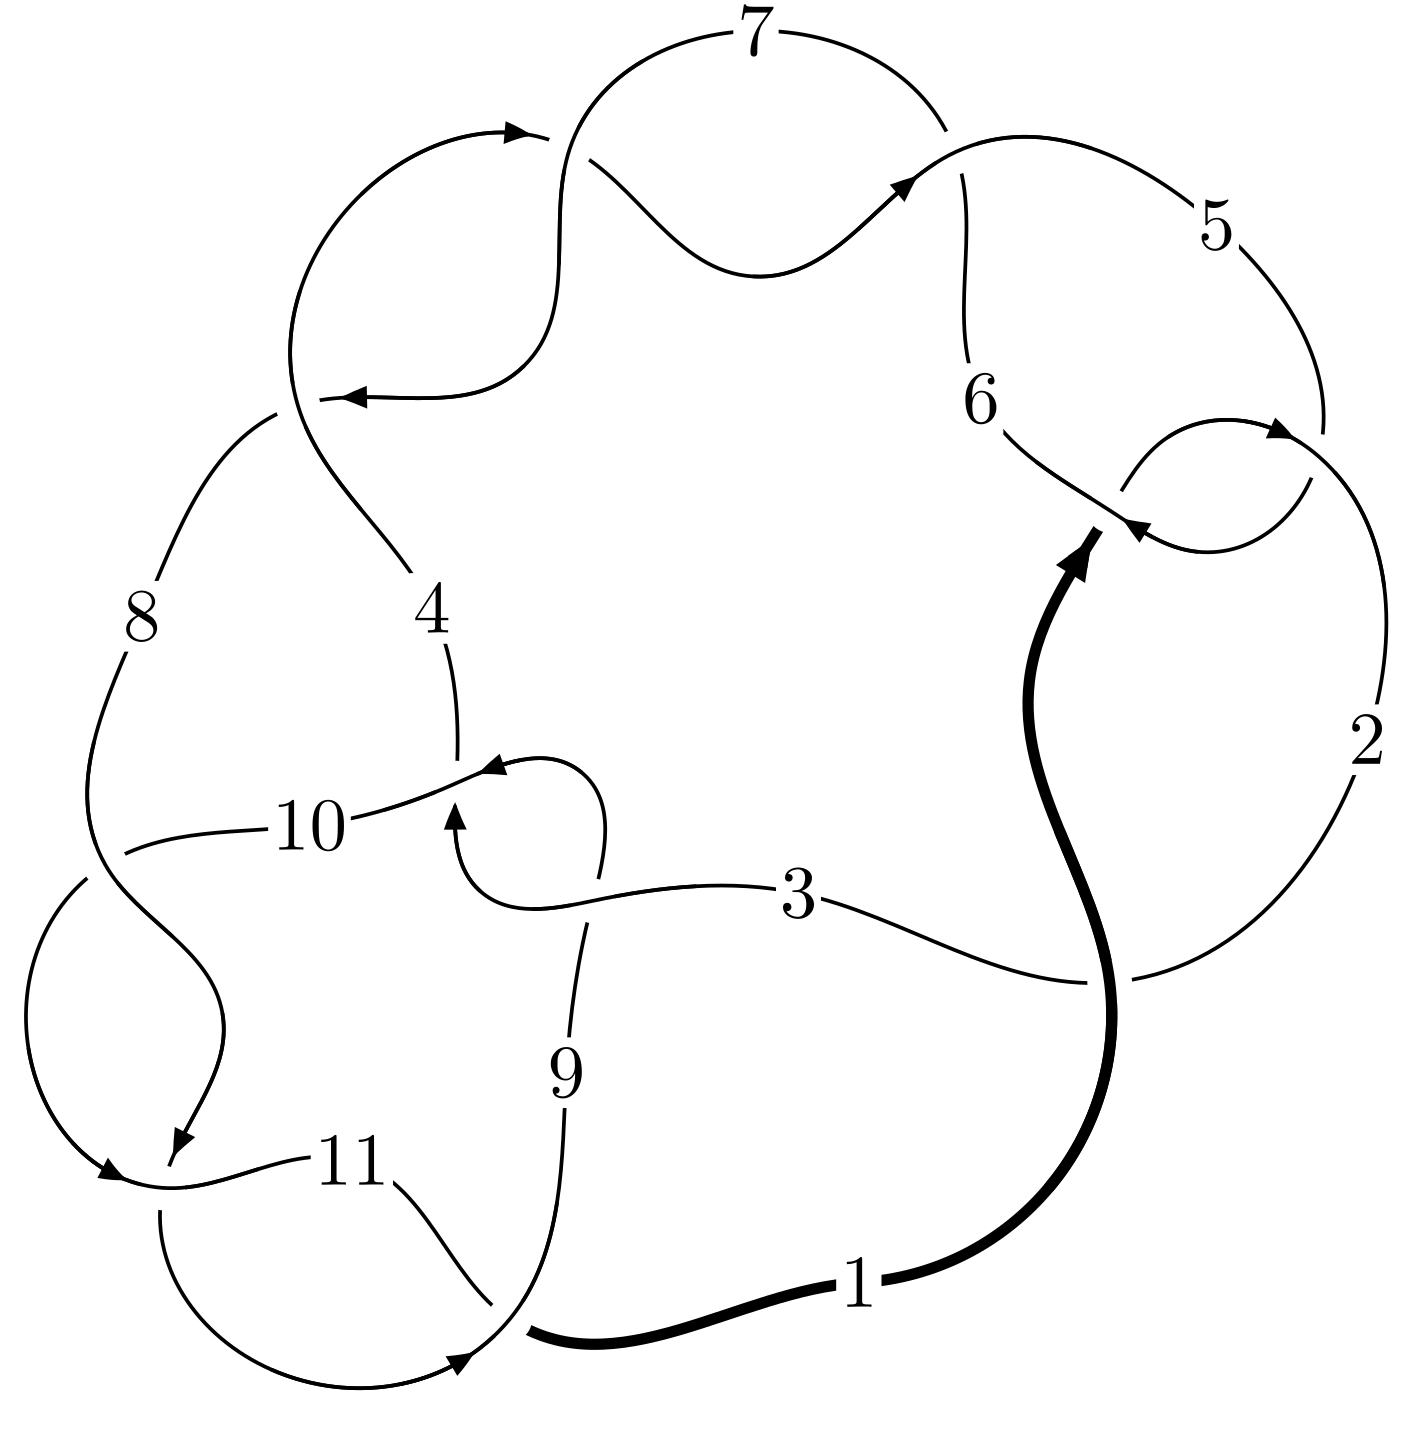
\includegraphics[width=112pt]{../../../GIT/diagram.site/Diagrams/png/410_11a_161.png}\\
\ \ \ A knot diagram\footnotemark}&
\allowdisplaybreaks
\textbf{Linearized knot diagam} \\
\cline{2-2}
 &
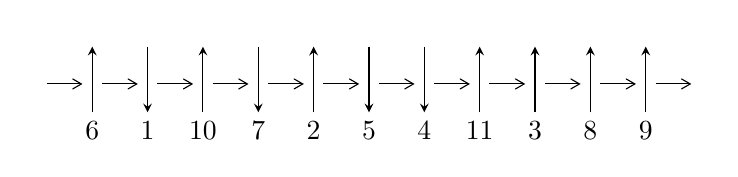
\begin{tikzpicture}[x=20pt, y=17pt]
	% nodes
	\node (C0) at (0, 0) {};
	\node (C1) at (1, 0) {};
	\node (C1U) at (1, +1) {};
	\node (C1D) at (1, -1) {6};

	\node (C2) at (2, 0) {};
	\node (C2U) at (2, +1) {};
	\node (C2D) at (2, -1) {1};

	\node (C3) at (3, 0) {};
	\node (C3U) at (3, +1) {};
	\node (C3D) at (3, -1) {10};

	\node (C4) at (4, 0) {};
	\node (C4U) at (4, +1) {};
	\node (C4D) at (4, -1) {7};

	\node (C5) at (5, 0) {};
	\node (C5U) at (5, +1) {};
	\node (C5D) at (5, -1) {2};

	\node (C6) at (6, 0) {};
	\node (C6U) at (6, +1) {};
	\node (C6D) at (6, -1) {5};

	\node (C7) at (7, 0) {};
	\node (C7U) at (7, +1) {};
	\node (C7D) at (7, -1) {4};

	\node (C8) at (8, 0) {};
	\node (C8U) at (8, +1) {};
	\node (C8D) at (8, -1) {11};

	\node (C9) at (9, 0) {};
	\node (C9U) at (9, +1) {};
	\node (C9D) at (9, -1) {3};

	\node (C10) at (10, 0) {};
	\node (C10U) at (10, +1) {};
	\node (C10D) at (10, -1) {8};

	\node (C11) at (11, 0) {};
	\node (C11U) at (11, +1) {};
	\node (C11D) at (11, -1) {9};
	\node (C12) at (12, 0) {};

	% arrows
	\draw[->,>={angle 60}]
	(C0) edge (C1) (C1) edge (C2) (C2) edge (C3) (C3) edge (C4) (C4) edge (C5) (C5) edge (C6) (C6) edge (C7) (C7) edge (C8) (C8) edge (C9) (C9) edge (C10) (C10) edge (C11) (C11) edge (C12) ;	\draw[->,>=stealth]
	(C1D) edge (C1U) (C2U) edge (C2D) (C3D) edge (C3U) (C4U) edge (C4D) (C5D) edge (C5U) (C6U) edge (C6D) (C7U) edge (C7D) (C8D) edge (C8U) (C9D) edge (C9U) (C10D) edge (C10U) (C11D) edge (C11U) ;
	\end{tikzpicture} \\
\hhline{~~} \\& 
\textbf{Solving Sequence} \\ \cline{2-2} 
 &
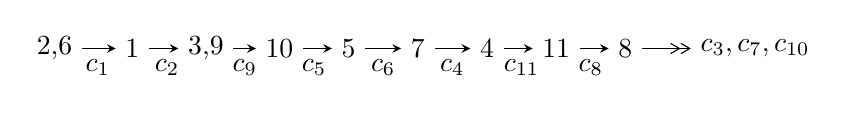
\begin{tikzpicture}[x=25pt, y=7pt]
	% node
	\node (A0) at (-1/8, 0) {2,6};
	\node (A1) at (1, 0) {1};
	\node (A2) at (33/16, 0) {3,9};
	\node (A3) at (25/8, 0) {10};
	\node (A4) at (33/8, 0) {5};
	\node (A5) at (41/8, 0) {7};
	\node (A6) at (49/8, 0) {4};
	\node (A7) at (57/8, 0) {11};
	\node (A8) at (65/8, 0) {8};
	\node (C1) at (1/2, -1) {$c_{1}$};
	\node (C2) at (3/2, -1) {$c_{2}$};
	\node (C3) at (21/8, -1) {$c_{9}$};
	\node (C4) at (29/8, -1) {$c_{5}$};
	\node (C5) at (37/8, -1) {$c_{6}$};
	\node (C6) at (45/8, -1) {$c_{4}$};
	\node (C7) at (53/8, -1) {$c_{11}$};
	\node (C8) at (61/8, -1) {$c_{8}$};
	\node (A9) at (10, 0) {$c_{3},c_{7},c_{10}$};

	% edge
	\draw[->,>=stealth]	
	(A0) edge (A1) (A1) edge (A2) (A2) edge (A3) (A3) edge (A4) (A4) edge (A5) (A5) edge (A6) (A6) edge (A7) (A7) edge (A8) ;
	\draw[->>,>={angle 60}]	
	(A8) edge (A9);
\end{tikzpicture} \\ 

\end{tabular} \\

\footnotetext{
The image of knot diagram is generated by the software ``\textbf{Draw programme}" developed by Andrew Bartholomew(\url{http://www.layer8.co.uk/maths/draw/index.htm\#Running-draw}), where we modified some parts for our purpose(\url{https://github.com/CATsTAILs/LinksPainter}).
}\phantom \\ \newline 
\centering \textbf{Ideals for irreducible components\footnotemark of $X_{\text{par}}$} 
 
\begin{align*}
I^u_{1}&=\langle 
- u^{20}-2 u^{18}+\cdots+b-2 u,\;u^{28}+u^{27}+\cdots+a+2,\;u^{32}+2 u^{31}+\cdots+4 u+1\rangle \\
I^u_{2}&=\langle 
u^2+b,\;- u^2+a+u,\;u^4- u^3+u^2+1\rangle \\
\\
\end{align*}
\raggedright * 2 irreducible components of $\dim_{\mathbb{C}}=0$, with total 36 representations.\\
\footnotetext{All coefficients of polynomials are rational numbers. But the coefficients are sometimes approximated in decimal forms when there is not enough margin.}
\newpage
\renewcommand{\arraystretch}{1}
\centering \section*{I. $I^u_{1}= \langle - u^{20}-2 u^{18}+\cdots+b-2 u,\;u^{28}+u^{27}+\cdots+a+2,\;u^{32}+2 u^{31}+\cdots+4 u+1 \rangle$}
\flushleft \textbf{(i) Arc colorings}\\
\begin{tabular}{m{7pt} m{180pt} m{7pt} m{180pt} }
\flushright $a_{2}=$&$\begin{pmatrix}1\\0\end{pmatrix}$ \\
\flushright $a_{6}=$&$\begin{pmatrix}0\\u\end{pmatrix}$ \\
\flushright $a_{1}=$&$\begin{pmatrix}1\\u^2\end{pmatrix}$ \\
\flushright $a_{3}=$&$\begin{pmatrix}u^2+1\\u^4\end{pmatrix}$ \\
\flushright $a_{9}=$&$\begin{pmatrix}- u^{28}- u^{27}+\cdots-6 u-2\\u^{20}+2 u^{18}+\cdots+2 u^2+2 u\end{pmatrix}$ \\
\flushright $a_{10}=$&$\begin{pmatrix}-2 u^{30}- u^{29}+\cdots-7 u-3\\2 u^{31}+4 u^{30}+\cdots+9 u+2\end{pmatrix}$ \\
\flushright $a_{5}=$&$\begin{pmatrix}- u\\u\end{pmatrix}$ \\
\flushright $a_{7}=$&$\begin{pmatrix}- u^3\\u^3+u\end{pmatrix}$ \\
\flushright $a_{4}=$&$\begin{pmatrix}- u^5- u\\u^5+u^3+u\end{pmatrix}$ \\
\flushright $a_{11}=$&$\begin{pmatrix}u^{30}+u^{29}+\cdots+7 u+3\\- u^{31}-2 u^{30}+\cdots-5 u-1\end{pmatrix}$ \\
\flushright $a_{8}=$&$\begin{pmatrix}- u^7-2 u^3\\u^7+u^5+2 u^3+u\end{pmatrix}$\\ \flushright $a_{8}=$&$\begin{pmatrix}- u^7-2 u^3\\u^7+u^5+2 u^3+u\end{pmatrix}$\\&\end{tabular}
\flushleft \textbf{(ii) Obstruction class $= -1$}\\~\\
\flushleft \textbf{(iii) Cusp Shapes $= 4 u^{31}+8 u^{30}+19 u^{29}+22 u^{28}+72 u^{27}+97 u^{26}+199 u^{25}+195 u^{24}+434 u^{23}+440 u^{22}+814 u^{21}+663 u^{20}+1230 u^{19}+979 u^{18}+1669 u^{17}+1135 u^{16}+1826 u^{15}+1208 u^{14}+1820 u^{13}+1120 u^{12}+1432 u^{11}+910 u^{10}+996 u^9+668 u^8+516 u^7+390 u^6+216 u^5+187 u^4+58 u^3+55 u^2+13 u+11$}\\~\\
\newpage\renewcommand{\arraystretch}{1}
\flushleft \textbf{(iv) u-Polynomials at the component}\newline \\
\begin{tabular}{m{50pt}|m{274pt}}
Crossings & \hspace{64pt}u-Polynomials at each crossing \\
\hline $$\begin{aligned}c_{1},c_{5}\end{aligned}$$&$\begin{aligned}
&u^{32}-2 u^{31}+\cdots-4 u+1
\end{aligned}$\\
\hline $$\begin{aligned}c_{2},c_{4},c_{6}\\c_{7}\end{aligned}$$&$\begin{aligned}
&u^{32}+6 u^{31}+\cdots-56 u^2+1
\end{aligned}$\\
\hline $$\begin{aligned}c_{3},c_{9}\end{aligned}$$&$\begin{aligned}
&u^{32}- u^{31}+\cdots+24 u-16
\end{aligned}$\\
\hline $$\begin{aligned}c_{8},c_{10},c_{11}\end{aligned}$$&$\begin{aligned}
&u^{32}+5 u^{31}+\cdots-4 u-1
\end{aligned}$\\
\hline
\end{tabular}\\~\\
\newpage\renewcommand{\arraystretch}{1}
\flushleft \textbf{(v) Riley Polynomials at the component}\newline \\
\begin{tabular}{m{50pt}|m{274pt}}
Crossings & \hspace{64pt}Riley Polynomials at each crossing \\
\hline $$\begin{aligned}c_{1},c_{5}\end{aligned}$$&$\begin{aligned}
&y^{32}+6 y^{31}+\cdots-56 y^2+1
\end{aligned}$\\
\hline $$\begin{aligned}c_{2},c_{4},c_{6}\\c_{7}\end{aligned}$$&$\begin{aligned}
&y^{32}+42 y^{31}+\cdots-112 y+1
\end{aligned}$\\
\hline $$\begin{aligned}c_{3},c_{9}\end{aligned}$$&$\begin{aligned}
&y^{32}-27 y^{31}+\cdots+448 y+256
\end{aligned}$\\
\hline $$\begin{aligned}c_{8},c_{10},c_{11}\end{aligned}$$&$\begin{aligned}
&y^{32}-35 y^{31}+\cdots-22 y+1
\end{aligned}$\\
\hline
\end{tabular}\\~\\
\newpage\flushleft \textbf{(vi) Complex Volumes and Cusp Shapes}
$$\begin{array}{c|c|c}  
\text{Solutions to }I^u_{1}& \I (\text{vol} + \sqrt{-1}CS) & \text{Cusp shape}\\
 \hline 
\begin{aligned}
u &= -0.213719 + 0.980461 I \\
a &= \phantom{-}0.92583 - 1.26296 I \\
b &= \phantom{-}0.082336 + 0.696499 I\end{aligned}
 & \phantom{-}4.40938 - 2.90320 I & \phantom{-}5.62644 + 3.88291 I \\ \hline\begin{aligned}
u &= -0.213719 - 0.980461 I \\
a &= \phantom{-}0.92583 + 1.26296 I \\
b &= \phantom{-}0.082336 - 0.696499 I\end{aligned}
 & \phantom{-}4.40938 + 2.90320 I & \phantom{-}5.62644 - 3.88291 I \\ \hline\begin{aligned}
u &= -0.644830 + 0.775185 I \\
a &= \phantom{-}2.23380 + 1.34488 I \\
b &= -0.42916 - 2.42515 I\end{aligned}
 & \phantom{-}4.97796 - 2.41324 I & \phantom{-}9.06378 + 3.46829 I \\ \hline\begin{aligned}
u &= -0.644830 - 0.775185 I \\
a &= \phantom{-}2.23380 - 1.34488 I \\
b &= -0.42916 + 2.42515 I\end{aligned}
 & \phantom{-}4.97796 + 2.41324 I & \phantom{-}9.06378 - 3.46829 I \\ \hline\begin{aligned}
u &= \phantom{-}0.798476 + 0.579251 I \\
a &= -1.76126 + 0.16137 I \\
b &= \phantom{-}0.88715 - 1.74244 I\end{aligned}
 & \phantom{-}10.60130 - 2.72339 I & \phantom{-}11.99326 + 0.76740 I \\ \hline\begin{aligned}
u &= \phantom{-}0.798476 - 0.579251 I \\
a &= -1.76126 - 0.16137 I \\
b &= \phantom{-}0.88715 + 1.74244 I\end{aligned}
 & \phantom{-}10.60130 + 2.72339 I & \phantom{-}11.99326 - 0.76740 I \\ \hline\begin{aligned}
u &= \phantom{-}0.601316 + 0.841196 I \\
a &= \phantom{-}0.867822 - 0.956388 I \\
b &= \phantom{-}0.193771 + 0.505942 I\end{aligned}
 & \phantom{-}2.73490 + 4.63620 I & \phantom{-}7.44058 - 7.48323 I \\ \hline\begin{aligned}
u &= \phantom{-}0.601316 - 0.841196 I \\
a &= \phantom{-}0.867822 + 0.956388 I \\
b &= \phantom{-}0.193771 - 0.505942 I\end{aligned}
 & \phantom{-}2.73490 - 4.63620 I & \phantom{-}7.44058 + 7.48323 I \\ \hline\begin{aligned}
u &= \phantom{-}0.645468 + 0.683845 I \\
a &= \phantom{-}0.0195996 - 0.1036640 I \\
b &= -0.539124 + 0.646751 I\end{aligned}
 & \phantom{-}3.24411 + 0.05063 I & \phantom{-}9.93222 + 0.12660 I \\ \hline\begin{aligned}
u &= \phantom{-}0.645468 - 0.683845 I \\
a &= \phantom{-}0.0195996 + 0.1036640 I \\
b &= -0.539124 - 0.646751 I\end{aligned}
 & \phantom{-}3.24411 - 0.05063 I & \phantom{-}9.93222 - 0.12660 I\\
 \hline 
 \end{array}$$\newpage$$\begin{array}{c|c|c}  
\text{Solutions to }I^u_{1}& \I (\text{vol} + \sqrt{-1}CS) & \text{Cusp shape}\\
 \hline 
\begin{aligned}
u &= \phantom{-}0.614078 + 0.966359 I \\
a &= -1.02310 + 2.02918 I \\
b &= -0.31554 - 2.13236 I\end{aligned}
 & \phantom{-}9.31106 + 7.91275 I & \phantom{-}9.40540 - 6.63145 I \\ \hline\begin{aligned}
u &= \phantom{-}0.614078 - 0.966359 I \\
a &= -1.02310 - 2.02918 I \\
b &= -0.31554 + 2.13236 I\end{aligned}
 & \phantom{-}9.31106 - 7.91275 I & \phantom{-}9.40540 + 6.63145 I \\ \hline\begin{aligned}
u &= -0.423229 + 0.733264 I \\
a &= -0.896141 - 0.367650 I \\
b &= \phantom{-}0.294342 + 0.546654 I\end{aligned}
 & \phantom{-}0.00047 - 1.65514 I & \phantom{-}0.39437 + 4.54470 I \\ \hline\begin{aligned}
u &= -0.423229 - 0.733264 I \\
a &= -0.896141 + 0.367650 I \\
b &= \phantom{-}0.294342 - 0.546654 I\end{aligned}
 & \phantom{-}0.00047 + 1.65514 I & \phantom{-}0.39437 - 4.54470 I \\ \hline\begin{aligned}
u &= -0.145430 + 0.769393 I \\
a &= -0.613814 + 1.208160 I \\
b &= \phantom{-}0.426833 - 0.149998 I\end{aligned}
 & -1.08342 - 1.49550 I & -1.76412 + 6.31671 I \\ \hline\begin{aligned}
u &= -0.145430 - 0.769393 I \\
a &= -0.613814 - 1.208160 I \\
b &= \phantom{-}0.426833 + 0.149998 I\end{aligned}
 & -1.08342 + 1.49550 I & -1.76412 - 6.31671 I \\ \hline\begin{aligned}
u &= \phantom{-}0.866691 + 0.917191 I \\
a &= -0.900315 + 0.319705 I \\
b &= \phantom{-}0.08960 - 1.43559 I\end{aligned}
 & \phantom{-}7.59385 + 3.21086 I & \phantom{-}2.30282 - 2.66372 I \\ \hline\begin{aligned}
u &= \phantom{-}0.866691 - 0.917191 I \\
a &= -0.900315 - 0.319705 I \\
b &= \phantom{-}0.08960 + 1.43559 I\end{aligned}
 & \phantom{-}7.59385 - 3.21086 I & \phantom{-}2.30282 + 2.66372 I \\ \hline\begin{aligned}
u &= -0.705788\phantom{ +0.000000I} \\
a &= -1.72336\phantom{ +0.000000I} \\
b &= \phantom{-}0.673766\phantom{ +0.000000I}\end{aligned}
 & \phantom{-}7.74304\phantom{ +0.000000I} & \phantom{-}12.4360\phantom{ +0.000000I} \\ \hline\begin{aligned}
u &= -0.918056 + 0.925441 I \\
a &= \phantom{-}0.220309 + 0.450379 I \\
b &= \phantom{-}0.124115 - 1.293980 I\end{aligned}
 & \phantom{-}12.49900 - 0.30826 I & \phantom{-}9.65224 - 0.25325 I\\
 \hline 
 \end{array}$$\newpage$$\begin{array}{c|c|c}  
\text{Solutions to }I^u_{1}& \I (\text{vol} + \sqrt{-1}CS) & \text{Cusp shape}\\
 \hline 
\begin{aligned}
u &= -0.918056 - 0.925441 I \\
a &= \phantom{-}0.220309 - 0.450379 I \\
b &= \phantom{-}0.124115 + 1.293980 I\end{aligned}
 & \phantom{-}12.49900 + 0.30826 I & \phantom{-}9.65224 + 0.25325 I \\ \hline\begin{aligned}
u &= -0.945672 + 0.902976 I \\
a &= -1.81639 - 0.29726 I \\
b &= \phantom{-}0.97029 + 3.38005 I\end{aligned}
 & -19.5223 + 4.2287 I & \phantom{-}11.43737 - 1.00370 I \\ \hline\begin{aligned}
u &= -0.945672 - 0.902976 I \\
a &= -1.81639 + 0.29726 I \\
b &= \phantom{-}0.97029 - 3.38005 I\end{aligned}
 & -19.5223 - 4.2287 I & \phantom{-}11.43737 + 1.00370 I \\ \hline\begin{aligned}
u &= \phantom{-}0.915023 + 0.941366 I \\
a &= \phantom{-}2.39534 - 0.89971 I \\
b &= -0.12103 + 4.15879 I\end{aligned}
 & \phantom{-}14.7168 + 3.3681 I & \phantom{-}10.32984 - 2.30184 I \\ \hline\begin{aligned}
u &= \phantom{-}0.915023 - 0.941366 I \\
a &= \phantom{-}2.39534 + 0.89971 I \\
b &= -0.12103 - 4.15879 I\end{aligned}
 & \phantom{-}14.7168 - 3.3681 I & \phantom{-}10.32984 + 2.30184 I \\ \hline\begin{aligned}
u &= -0.903860 + 0.952544 I \\
a &= \phantom{-}1.222940 + 0.282890 I \\
b &= -0.231803 - 1.207090 I\end{aligned}
 & \phantom{-}12.41050 - 6.40086 I & \phantom{-}9.40627 + 4.90251 I \\ \hline\begin{aligned}
u &= -0.903860 - 0.952544 I \\
a &= \phantom{-}1.222940 - 0.282890 I \\
b &= -0.231803 + 1.207090 I\end{aligned}
 & \phantom{-}12.41050 + 6.40086 I & \phantom{-}9.40627 - 4.90251 I \\ \hline\begin{aligned}
u &= -0.900364 + 0.984023 I \\
a &= -1.99724 - 1.52148 I \\
b &= -0.77261 + 3.46344 I\end{aligned}
 & \phantom{-}19.6887 - 11.0126 I & \phantom{-}11.01976 + 5.54593 I \\ \hline\begin{aligned}
u &= -0.900364 - 0.984023 I \\
a &= -1.99724 + 1.52148 I \\
b &= -0.77261 - 3.46344 I\end{aligned}
 & \phantom{-}19.6887 + 11.0126 I & \phantom{-}11.01976 - 5.54593 I \\ \hline\begin{aligned}
u &= \phantom{-}0.161526 + 0.565105 I \\
a &= \phantom{-}0.28634 - 2.32243 I \\
b &= -0.713364 + 0.589378 I\end{aligned}
 & \phantom{-}1.29270 + 0.72541 I & \phantom{-}4.11413 + 2.96939 I\\
 \hline 
 \end{array}$$\newpage$$\begin{array}{c|c|c}  
\text{Solutions to }I^u_{1}& \I (\text{vol} + \sqrt{-1}CS) & \text{Cusp shape}\\
 \hline 
\begin{aligned}
u &= \phantom{-}0.161526 - 0.565105 I \\
a &= \phantom{-}0.28634 + 2.32243 I \\
b &= -0.713364 - 0.589378 I\end{aligned}
 & \phantom{-}1.29270 - 0.72541 I & \phantom{-}4.11413 - 2.96939 I \\ \hline\begin{aligned}
u &= -0.309046\phantom{ +0.000000I} \\
a &= -0.604076\phantom{ +0.000000I} \\
b &= -0.565378\phantom{ +0.000000I}\end{aligned}
 & \phantom{-}0.870053\phantom{ +0.000000I} & \phantom{-}11.8550\phantom{ +0.000000I}\\
 \hline 
 \end{array}$$\newpage\newpage\renewcommand{\arraystretch}{1}
\centering \section*{II. $I^u_{2}= \langle u^2+b,\;- u^2+a+u,\;u^4- u^3+u^2+1 \rangle$}
\flushleft \textbf{(i) Arc colorings}\\
\begin{tabular}{m{7pt} m{180pt} m{7pt} m{180pt} }
\flushright $a_{2}=$&$\begin{pmatrix}1\\0\end{pmatrix}$ \\
\flushright $a_{6}=$&$\begin{pmatrix}0\\u\end{pmatrix}$ \\
\flushright $a_{1}=$&$\begin{pmatrix}1\\u^2\end{pmatrix}$ \\
\flushright $a_{3}=$&$\begin{pmatrix}u^2+1\\u^3- u^2-1\end{pmatrix}$ \\
\flushright $a_{9}=$&$\begin{pmatrix}u^2- u\\- u^2\end{pmatrix}$ \\
\flushright $a_{10}=$&$\begin{pmatrix}u^2- u\\- u^2\end{pmatrix}$ \\
\flushright $a_{5}=$&$\begin{pmatrix}- u\\u\end{pmatrix}$ \\
\flushright $a_{7}=$&$\begin{pmatrix}- u^3\\u^3+u\end{pmatrix}$ \\
\flushright $a_{4}=$&$\begin{pmatrix}u^2+1\\u^3- u^2-1\end{pmatrix}$ \\
\flushright $a_{11}=$&$\begin{pmatrix}u^2- u+1\\0\end{pmatrix}$ \\
\flushright $a_{8}=$&$\begin{pmatrix}-1\\- u^2\end{pmatrix}$\\ \flushright $a_{8}=$&$\begin{pmatrix}-1\\- u^2\end{pmatrix}$\\&\end{tabular}
\flushleft \textbf{(ii) Obstruction class $= 1$}\\~\\
\flushleft \textbf{(iii) Cusp Shapes $= -5 u^2+6 u+7$}\\~\\
\newpage\renewcommand{\arraystretch}{1}
\flushleft \textbf{(iv) u-Polynomials at the component}\newline \\
\begin{tabular}{m{50pt}|m{274pt}}
Crossings & \hspace{64pt}u-Polynomials at each crossing \\
\hline $$\begin{aligned}c_{1}\end{aligned}$$&$\begin{aligned}
&u^4- u^3+u^2+1
\end{aligned}$\\
\hline $$\begin{aligned}c_{2},c_{6},c_{7}\end{aligned}$$&$\begin{aligned}
&u^4+u^3+3 u^2+2 u+1
\end{aligned}$\\
\hline $$\begin{aligned}c_{3},c_{9}\end{aligned}$$&$\begin{aligned}
&u^4
\end{aligned}$\\
\hline $$\begin{aligned}c_{4}\end{aligned}$$&$\begin{aligned}
&u^4- u^3+3 u^2-2 u+1
\end{aligned}$\\
\hline $$\begin{aligned}c_{5}\end{aligned}$$&$\begin{aligned}
&u^4+u^3+u^2+1
\end{aligned}$\\
\hline $$\begin{aligned}c_{8}\end{aligned}$$&$\begin{aligned}
&(u+1)^4
\end{aligned}$\\
\hline $$\begin{aligned}c_{10},c_{11}\end{aligned}$$&$\begin{aligned}
&(u-1)^4
\end{aligned}$\\
\hline
\end{tabular}\\~\\
\newpage\renewcommand{\arraystretch}{1}
\flushleft \textbf{(v) Riley Polynomials at the component}\newline \\
\begin{tabular}{m{50pt}|m{274pt}}
Crossings & \hspace{64pt}Riley Polynomials at each crossing \\
\hline $$\begin{aligned}c_{1},c_{5}\end{aligned}$$&$\begin{aligned}
&y^4+y^3+3 y^2+2 y+1
\end{aligned}$\\
\hline $$\begin{aligned}c_{2},c_{4},c_{6}\\c_{7}\end{aligned}$$&$\begin{aligned}
&y^4+5 y^3+7 y^2+2 y+1
\end{aligned}$\\
\hline $$\begin{aligned}c_{3},c_{9}\end{aligned}$$&$\begin{aligned}
&y^4
\end{aligned}$\\
\hline $$\begin{aligned}c_{8},c_{10},c_{11}\end{aligned}$$&$\begin{aligned}
&(y-1)^4
\end{aligned}$\\
\hline
\end{tabular}\\~\\
\newpage\flushleft \textbf{(vi) Complex Volumes and Cusp Shapes}
$$\begin{array}{c|c|c}  
\text{Solutions to }I^u_{2}& \I (\text{vol} + \sqrt{-1}CS) & \text{Cusp shape}\\
 \hline 
\begin{aligned}
u &= -0.351808 + 0.720342 I \\
a &= -0.043315 - 1.227190 I \\
b &= \phantom{-}0.395123 + 0.506844 I\end{aligned}
 & \phantom{-}1.43393 - 1.41510 I & \phantom{-}6.86477 + 6.85627 I \\ \hline\begin{aligned}
u &= -0.351808 - 0.720342 I \\
a &= -0.043315 + 1.227190 I \\
b &= \phantom{-}0.395123 - 0.506844 I\end{aligned}
 & \phantom{-}1.43393 + 1.41510 I & \phantom{-}6.86477 - 6.85627 I \\ \hline\begin{aligned}
u &= \phantom{-}0.851808 + 0.911292 I \\
a &= -0.956685 + 0.641200 I \\
b &= \phantom{-}0.10488 - 1.55249 I\end{aligned}
 & \phantom{-}8.43568 + 3.16396 I & \phantom{-}12.63523 - 2.29471 I \\ \hline\begin{aligned}
u &= \phantom{-}0.851808 - 0.911292 I \\
a &= -0.956685 - 0.641200 I \\
b &= \phantom{-}0.10488 + 1.55249 I\end{aligned}
 & \phantom{-}8.43568 - 3.16396 I & \phantom{-}12.63523 + 2.29471 I\\
 \hline 
 \end{array}$$\newpage
\newpage\renewcommand{\arraystretch}{1}
\centering \section*{ III. u-Polynomials}
\begin{tabular}{m{50pt}|m{274pt}}
Crossings & \hspace{64pt}u-Polynomials at each crossing \\
\hline $$\begin{aligned}c_{1}\end{aligned}$$&$\begin{aligned}
&(u^4- u^3+u^2+1)(u^{32}-2 u^{31}+\cdots-4 u+1)
\end{aligned}$\\
\hline $$\begin{aligned}c_{2},c_{6},c_{7}\end{aligned}$$&$\begin{aligned}
&(u^4+u^3+3 u^2+2 u+1)(u^{32}+6 u^{31}+\cdots-56 u^2+1)
\end{aligned}$\\
\hline $$\begin{aligned}c_{3},c_{9}\end{aligned}$$&$\begin{aligned}
&u^4(u^{32}- u^{31}+\cdots+24 u-16)
\end{aligned}$\\
\hline $$\begin{aligned}c_{4}\end{aligned}$$&$\begin{aligned}
&(u^4- u^3+3 u^2-2 u+1)(u^{32}+6 u^{31}+\cdots-56 u^2+1)
\end{aligned}$\\
\hline $$\begin{aligned}c_{5}\end{aligned}$$&$\begin{aligned}
&(u^4+u^3+u^2+1)(u^{32}-2 u^{31}+\cdots-4 u+1)
\end{aligned}$\\
\hline $$\begin{aligned}c_{8}\end{aligned}$$&$\begin{aligned}
&((u+1)^4)(u^{32}+5 u^{31}+\cdots-4 u-1)
\end{aligned}$\\
\hline $$\begin{aligned}c_{10},c_{11}\end{aligned}$$&$\begin{aligned}
&((u-1)^4)(u^{32}+5 u^{31}+\cdots-4 u-1)
\end{aligned}$\\
\hline
\end{tabular}\newpage\renewcommand{\arraystretch}{1}
\centering \section*{ IV. Riley Polynomials}
\begin{tabular}{m{50pt}|m{274pt}}
Crossings & \hspace{64pt}Riley Polynomials at each crossing \\
\hline $$\begin{aligned}c_{1},c_{5}\end{aligned}$$&$\begin{aligned}
&(y^4+y^3+3 y^2+2 y+1)(y^{32}+6 y^{31}+\cdots-56 y^2+1)
\end{aligned}$\\
\hline $$\begin{aligned}c_{2},c_{4},c_{6}\\c_{7}\end{aligned}$$&$\begin{aligned}
&(y^4+5 y^3+7 y^2+2 y+1)(y^{32}+42 y^{31}+\cdots-112 y+1)
\end{aligned}$\\
\hline $$\begin{aligned}c_{3},c_{9}\end{aligned}$$&$\begin{aligned}
&y^4(y^{32}-27 y^{31}+\cdots+448 y+256)
\end{aligned}$\\
\hline $$\begin{aligned}c_{8},c_{10},c_{11}\end{aligned}$$&$\begin{aligned}
&((y-1)^4)(y^{32}-35 y^{31}+\cdots-22 y+1)
\end{aligned}$\\
\hline
\end{tabular}
\vskip 2pc
\end{document}